\documentclass[11pt,letter, swedish, english
]{article}
\pdfoutput=1

\usepackage{../custom_as}

\graphicspath{ {plots/} }


%%Drar in tabell och figurtexter
\usepackage[margin=10 pt]{caption}
%%För att lägga in 'att göra'-noteringar i texten
\usepackage{todonotes} %\todo{...}

%%För att själv bestämma marginalerna. 
\usepackage[
%            top    = 3cm,
%            bottom = 3cm,
%            left   = 3cm, right  = 3cm
]{geometry}


\swapcommands{\Pi}{\varPi}

\DeclareMathAlphabet{\mathpzc}{OT1}{pzc}{m}{it}
\newcommand{\oh}{\ensuremath\mathpzc{o}}

\newcommand{\Ei}{\ensuremath\mathrm{Ei}}

\begin{document}

%%%%%%%%%%%%%%%%% vvv Inbyggd titelsida vvv %%%%%%%%%%%%%%%%%
% \begin{titlepage}
\title{Asymptotic Analasys and Pertubation Theory -- AMATH\,732 \\
Assignment 2}
\author{Andréas Sundström}
\date{\today}

\maketitle

%%%%%%%%%%%%%%%%% ^^^ Inbyggd titelsida ^^^ %%%%%%%%%%%%%%%%%

%Om man vill ha en lista med vilka todo:s som finns.
%\todolist

\section{Dimensional analysis from Lin\,\&\,Segel}
\setcounter{subsection}{4}
\renewcommand{\thesubsection}{L\&S 6.2: \arabic{subsection}}
\subsection{Ship propeller}
A ship popeller's thurst $T$ depends on it's radius $a$, the number of
revolutions per minute $n$, the velocity $V$, the acceleration of
gravity $g$, the water's density $\rho$ and kinematic viscosity $\nu$.
We're tasked to use formal dimensinal analysis to show that
\begin{equation}
\frac{T}{\rho a^2 V^2} = 
\varphi\qty(\frac{an}{V}, \frac{aV}{\nu}, \frac{ag}{V^2}).
\end{equation}

To begin with, we list all the parameters' dimensions:
\begin{equation}
\begin{aligned}
[T]=[\mathcal{LMT}^{-2}]\qcomma [a]=[\mathcal{L}]
&\qcomma [n]=[\mathcal{T}^{-1}]\qcomma [V]=[\mathcal{LT}^{-1}]\\
[g]=[\mathcal{LT}^{-2}]\qcomma [\nu]=&[\mathcal{L}^2\mathcal{T}^{-1}]
\qcomma  [\rho]=[\mathcal{ML}^{-3}].
\end{aligned}
\end{equation}
With the dimensions of all the parameters listed we can begin
creating dimension less parameters
\begin{equation}
\Pi_i = a^{A_i}n^{B_i} V^{C_i} g^{D_i} \nu^{E_i}\rho^{F_i} T^{G_i} \qcomma
[\Pi_i] = [1].
\end{equation}
This is no more than a linear system of equations, one equation for
each fundamental dimension,
\begin{equation}\label{eq:1_dim_matrix}
\begin{pmatrix}
0&0&0&0&0&1&1\\
1&0&1&1&2&-3&1\\
0&-1&-1&-2&-1&0&-2
\end{pmatrix}
\begin{pmatrix}
A_i\\B_i\\C_i\\D_i\\E_i\\F_i\\G_i
\end{pmatrix}
=\begin{pmatrix}
0\\0\\0
\end{pmatrix}.
\end{equation}
Here the rows represents the dimensions of mass, length and time respectivley.
We have three equations and seven unknowns, so we have four free
parameters. 

Since we were given a set relation to prove it's easy to confirm that
the relation satisfies \eqref{eq:1_dim_matrix}, but if we were to find
a relationship on our own we would now need to choose which of the
parameters to be free. A good choice would be to let $G_i=\Gamma_i$ be free and
only have the value $1$ once and the rest of the time be $0$. The
other free parameters can be chosen more freely; in lack of a beter
choice, pick $A_i=\alpha_i$, $B_i=\beta_i$ and $C_i=\gamma_i$ to be
the free parameters. 
This gives us the equations
\begin{equation}
\begin{cases}
F_i=-\Gamma_i\\
D_i+2E_i-3F_i=-\alpha_i-\gamma_i-\Gamma_i\\
2D_i+E_i=-\beta_i-\gamma_i-2\Gamma_i,
\end{cases}
\Longleftrightarrow
\begin{cases}
F_i=-\Gamma_i\\
D_i+2E_i=-\alpha_i-\gamma_i-4\Gamma_i\\
2D_i+E_i=-\beta_i-\gamma_i-2\Gamma_i.
\end{cases}
\end{equation}

From here it's just a matter of choosing values for the free
parameters. One such choice would be $\Gamma_i=(1, 0, 0, 0)$, 
$\alpha_i=(-2, 1, 1, 1)$, $\beta_i=(0, 1, 0, 0)$ and
$\gamma_i=(-2, -1, 1, -2)$, giving us $D_i=(0, 0, 0, 1)$, 
$E_i=(0, 0, -1, 0)$ and $F_i=-\Gamma_i$.
The set of Buckingham $\Pi$
parameters now becomes
\begin{equation}
\Pi_1=\frac{T}{\rho a^2V^2}\qcomma \Pi_2=\frac{an}{V}\qcomma
\Pi_3=\frac{aV}{\nu}\qcomma \Pi_4=\frac{ag}{V^2}.
\end{equation}
\qed

\subsection{Diffusion and Brownian motion}
Here we're supposed to find that
\begin{equation}
D\propto\frac{kT}{a\mu},
\end{equation}
where $D$ is the diffusion constant, $k$ is the Boltzmann constant,
$T$ is the temperature, $a$ the radius of the paricles, and $\mu$ the
viscosity. The dimensions are
\begin{equation}
[D]=[\mathcal{L}^2\mathcal{T}^{-1}]\qcomma [k]=[\mathcal{ML}^2\mathcal{T}^{-2}\Theta^{-1}]\qcomma 
[T]=[\Theta]\qcomma 
[a]=[\mathcal{L}]\qcomma [\mu]=[\mathcal{ML}^{-1}\mathcal{T}^{-1}].
\end{equation}

Instead of doing the formal approach, as above, it's some times easier
to go ahead and eliminate one dimension after the other without
having to first set up all the equations. For instance we must have the
combination $kT$ to eliminate the temperature dimension; then mass can
be eliminated by dividing with $\mu$. By now, only the time and length
dimensions are left, and the only parameters left are $D$ and $a$. 

To eliminate time, we see that
\begin{equation}
\qty[\frac{kT}{\mu}] = \qty[\mathcal{L}^3\mathcal{T}^{-1}],
\end{equation}
which means that dividing by $D$ would eliminate the time
dimension. And finally we need to divinde by $a$ to get rid of the
length dimension, leaving us with the only Buckingham $\Pi$ parameter
\begin{equation}
\Pi=\frac{kT}{Da\mu} = ``\varphi(1)\text{''}.
\end{equation}
Or in other words
\begin{equation}
D=\text{const.}\times\frac{kT}{a\mu}.
\end{equation}
\qed



\section{Scaling from Lin\,\&\,Segel}
\setcounter{subsection}{1}
\renewcommand{\thesubsection}{L\&S 6.3: \arabic{subsection}}
\subsection{Scaling of an exponential function}
Here we're looking at the scale of the function
\begin{equation}
u^*(x^*)=A\ee^{-ax^*}\qcomma x\in I=[b, \infty)
\end{equation}
satisfying some first order ODE. The scaled quantities are $u=u^*/U$
and $x=x^*/L$. 

By following procedures to ensure that the scaled quantities shoud be
$\mathcal{O}_M(1)$, we get
\begin{equation}
U=\max_I\abs{u^*}=A\ee^{-ab},
\end{equation}
and 
\begin{equation}
\frac{U}{L}=\max_I\abs{\dv{u^*}{x^*}}=aA\ee^{-ab} \Longrightarrow
L=\frac{1}{a}.
\end{equation}

We see that the lengthscale $L$ is independent of $b$. This is because
the lengthscale should reflect the change in $x^*$ needed to change
$u^*$ by aome significant amount. And since the function is
exponential, $u^*$ will change by a factor of $\ee^{-1}$ for every
step of $\nicefrac{1}{a}$ that $x^*$ takes, regardless of where $x^*$
had it's origin. 

\subsection{Scaling with multiple independent variables}
Here we have some first order PDE with two indepedent variables $x^*$
and $y^*$, and one dependent variable $u^*$. The PDE governs the
behaviour in some domain $\mathcal{D}$. The scaled terms are
$u=u^*/U$, $x=x^*/L_x$ and $y=y^*/L_y$.

The scaling should stil be so that the scaled quantities are
$\mathcal{O}_M(1)$. Wherefore we still get
\begin{equation}
U=\max_\mathcal{D}\abs{u^*},
\end{equation}
and
\begin{equation}
\frac{U}{L_x}=\max_\mathcal{D}\abs{\pdv{u^*}{x^*}}\qcomma
\frac{U}{L_y}=\max_\mathcal{D}\abs{\pdv{u^*}{y^*}}.
\end{equation}


\subsection{Scaling with multiple dependent variables}
This is basically the same as above, but with two dependent variables
$u^*$ and $v^*$. With the same condition thet the scaled parameters
should be at most $\mathcal{O}_M(1)$, we get
\begin{equation}
U=\max_\mathcal{D}\abs{u^*} \qcomma
V=\max_\mathcal{D}\abs{v^*},
\end{equation}
and 
\begin{equation}
L_x=\max\qty{
U\qty(\max_\mathcal{D}\abs{\pdv{u^*}{x^*}})^{-1},\;
V\qty(\max_\mathcal{D}\abs{\pdv{v^*}{x^*}})^{-1}
}
\end{equation}
and $L_y$ is analogous to $L_x$.


\renewcommand{\thesubsection}{\arabic{section} (\alph{subsection})}
\renewcommand{\thesubsubsection}{\arabic{section} (\alph{subsection},\,\roman{subsubsection})}

\section{The Pythagorean theorem from dimensional analysis}
One way to prove the Pythagorean theorem is to use dimensional
analysis. 

\begin{figure}\centering
\resizebox{.5\textwidth}{!}{
\input{plots/right_triangle.pdf_t}}
\caption{A right triangle with a perpendicular droped from the
  hypotenuse to tha right angled vertex. The important thing to note
  here is that the two smaller triangles are both similar to the
  original one. }
\label{fig:triangle}
\end{figure}

Since any right triangle is determined by two independent
parameters, any properties of a right triangle can be expressed in
terms of the two independent parameters. For instance the total area
of the triangle in \figref{fig:triangle} can be given by
\begin{equation}
A_\text{tot}=:A_c=\tilde{f}(c, \theta).
\end{equation}
Here's where the dimensional analysis comes in. Since
$[A_c]=[\mathcal{L}^2]$, $[c]=[\mathcal{L}]$ and $[\theta]=[1]$, we
can write
\begin{equation}
\frac{A_c}{c^2}=f(\theta)
\quad\Longleftrightarrow\quad
A_c=c^2\,f(\theta)
\end{equation}
for some unknown function $f$. 

Now to the main twist. By dropping a perpendicular from the hypotenuse
to the right angled vertex, we get wo new triangles which are both
similar to the original triangle. Therefore
\begin{equation}
A_a=a^2f(\theta) \qcomma\text{and}\quad A_b=b^2f(\theta),
\end{equation}
for the exact same function $f$ and angle $\theta$. But since the
total area of the triangle is the sum of the areas of the smaller
one's, $A_c=A_a+A_b$, we must have
\begin{equation}
c^2f(\theta)=a^2f(\theta)+b^2f(\theta) \quad\Longleftrightarrow\quad 
c^2=a^2+b^2.
\end{equation}
\qed


\section{The projectile problem with air resitance}
Once again we take a look at the projectile problem, but this time
it's with air recistance and constant gravity. The prblem now becomes
\begin{equation}\label{eq:4_gov_eqn}
\frac{\dd^2{x^*}}{\dd{t^*}^2} + \frac{k}{m}\frac{\dd{x^*}}{\dd{t^*}} + g = 0
\qcomma x^*(0)=0\qcomma \eval{\dv{x^*}{t^*}}_{t^*=0}=v.
\end{equation}

\subsection{Scaling}
With $v$ suficiently small, the change in the maximum height won't be
too great from if there would be no drag. Hence the scale for $x$
should be $x=x^*/U$, with 
\begin{equation}\label{eq:4_xscale}
U=v^2/g\approx2\max(x)
\end{equation}
for small $v$'s. 
The time scale won't change much from the reduced problem either for
$v$ small enough. There are however an other argument for this. 

Consider the recipie for choosing the timescale:
\begin{equation}\label{eq:4_t_scale}
T=\min_{i\in\{1, 2\}}\qty{\qty[
U\times\qty(\max\abs{\frac{\dd^i x^*}{\dd{t^*}^i}})^{-1}
]^{\nicefrac{1}{i}}}
\end{equation}
and since $v=\max\abs{\dv{x^*}{t^*}}$ is small, \eqref{eq:4_t_scale}
tells us that we should choose the time scale based on the second
derivative. Therefore
\begin{equation}\label{eq:4_tscale}
T=\qty[\frac{v^2}{g}\times(g)^{-1}]^{\nicefrac{1}{2}} = \frac{v}{g}.
\end{equation}

\subsection{Non-dimensionalize}
We non-dimensionalize the problem by taking $x=x^*/U$ and $t=t^*/T$,
with $U$ and $T$ from \eqref{eq:4_xscale} and \eqref{eq:4_tscale}
respectively. Now the governing equation becomes
\begin{equation}
\frac{v^2}{g}\qty(\frac{v}{g})^{-2}\dv[2]{x}{t} 
+ \frac{k}{m} \frac{v^2}{g}\qty(\frac{v}{g})^{-1}\dv{x}{t}
+ g = 0,
\end{equation}
which when simplified gives us the analouge of \eqref{eq:4_gov_eqn}:
\begin{equation}
\dv[2]{x}{t} + \beta\dv{x}{t} + 1 = 0\qcomma
x(0)=0\qcomma \dot{x}(0)=1.
\end{equation}
Here $\beta=\frac{kv}{mg}$ is the maximum quitent between the
dragforce and the gravitational force on the projectile. Since we're
studying slow projectiles we know that $\beta$ is small, meaning that
gravity will always be the dominating force on the object. 

\subsection{Approximate solution and time to reach maximum height}
\subsubsection{Approximate solution}
To find an approximate solution with pertubation methods, expand
\begin{equation}
x(t, \beta) = x_0(t) + x_1(t)\beta + x_2(t)\beta^2 + \ldots.
\end{equation}
Substitution into the ODE and collection of powers of $\beta$ yiels
\begin{equation}
\ddot{x}_0+g + \beta\qty(\ddot{x}_1+\dot{x}_0) +
\beta^2\qty(\ddot{x}_2 + \dot{x}_1) + \ldots = 0.
\end{equation}
And the initial conditions are $x_i(0)=0$ for all $i$, and
$\dot{x}_i=0$ for $i\neq0$ and $\dot{x}_0=1$. Now we can solve for
each coefficient of $\beta^i$:
\vspace{-1mm}
\begin{enumerate}[label=$\order{\beta^{\arabic*}}$: , start=0, leftmargin=2cm]
\item $\displaystyle \ddot{x}_0=-g_{\phantom{0}} \quad\Longrightarrow\quad
x_0(t) = t - \frac{t^2}{2}$.
\item $\displaystyle \ddot{x}_1=-\dot{x}_0 \quad\Longrightarrow\quad
x_1(t) = \frac{t^3}{6} - \frac{t^2}{2}$.
\item $\displaystyle \ddot{x}_2=-\dot{x}_1 \quad\Longrightarrow\quad
x_2(t) = \frac{t^3}{6} - \frac{t^4}{24}$.
\end{enumerate}
Together we get\footnotemark{}
\begin{equation}\label{eq:4_xapprox}
x(t, \beta) = t - \frac{t^2}{2} + \beta\qty(\frac{t^3}{6}-\frac{t^2}{2})
 + \beta^2\qty(\frac{t^3}{6}-\frac{t^4}{24}) + \order{\beta^3}.
\end{equation}
\qed
\footnotetext{The error is bounded by $\order{\beta^3}$ due to the
  fact that all coefficients for the $\beta$'s are all polynomials in
  $t$ and $t$ is bounden during the period of interest. }

\subsubsection{Approximate time to reach maximum height}
To find an approximation of th time it takes for the projectile to
reach it's maximum height, $\tau$, we just differentiate $x$ from
\eqref{eq:4_xapprox} with respect to $t$ set that to $0$:
\begin{equation}
\begin{aligned}
1-\tau + \beta\qty(-\tau+\frac{\tau^2}{2}) 
+ \beta^2\qty(\frac{\tau^2}{2}-\frac{\tau^3}{6}) &= 0\\
\Longrightarrow\quad
1 - (1+\beta)\tau + \frac{\beta}{2}\qty(\beta -1)\tau^2 
- \frac{\beta^2}{6}\tau^3 &= 0
\end{aligned}
\end{equation}
To solve this equation, we use pertubation methods. 

Expand,
\begin{equation}
\tau(\beta) = \tau_0 + \tau_1\beta + \tau_2\beta^2 +\ldots,
\end{equation}
and insert into the polynomial. 
\begin{equation}
\begin{aligned}
0=&1 - (1+\beta)\qty(\tau_0+\tau_1\beta + \tau_2\beta^2+\ldots)\\
&+ \frac{\beta}{2}\qty(\beta -1)\qty(\tau_0^2+2\tau_0\tau_1\beta+\ldots)
+\frac{\beta^2}{6}\qty(\tau_0^3+\ldots) + \ldots.
\end{aligned}
\end{equation}
Collecting like powers of $\beta$
yields
\begin{enumerate}[label=$\order{\beta^{\arabic*}}$: , start=0, leftmargin=2cm]
\item $\displaystyle 1-\tau_0 = 0 \quad\Longrightarrow\quad
\tau_0=1$.
\item $\displaystyle -\tau_0-\tau_1+\frac{\tau_0}{2} = 0 \quad\Longrightarrow\quad
\tau_1= -\frac{\tau_0}{2} = -\frac{1}{2}$.
\item $\displaystyle -\tau_1-\tau_2+\frac{\tau_0^2}{2}-\tau_0\tau_1 -\frac{\tau_0^3}{6}= 0 \quad\Longrightarrow\quad
\tau_2=-\tau_1+\frac{\tau_0^2}{2}-\tau_0\tau_1 -\frac{\tau_0^3}{6} = \frac{4}{3}$.
\end{enumerate}
Therefore the time at which the projectile reaches it's maximum height
is 
\begin{equation}
\tau(\beta) = 1 - \frac{1}{2}\beta + \frac{5}{3}\beta^2 + \order{\beta^3}.
\end{equation}

To find the maximum height, just plug the expression for $\tau$ into
\begin{equation}
x_\text{max} = x\Big(\tau(\beta), \beta\Big)=\ldots
=\frac{1}{2}-\frac{\beta}{3} + \frac{\beta^2}{4} +\order{\beta^3}
\end{equation}

\qed



\section{A piano wire}
\newcommand{\yn}{\ensuremath{}y^{(n)}}

An ideal (no bending stiffness) piano wire is governed by the equation
\begin{equation}
\rho A \pdv[2]{y}{{t^*}} - T\pdv[2]{y}{{x^*}} = 0 \qcomma 0\le x^*\le L,
\end{equation}
together with the boundry conditions $y(0)=y(L)=0$. Here $\rho A$ is
the mass density per unit length and $T$ is the tension in the
string. This PDE has solutions of the form
\begin{equation}
\yn=\ee^{-\ii\omega_n^*t^*}\sin(n\pi\frac{x^*}{L}).
\end{equation}
Since we're dealing with a linear PDE with constant coefficients, the
solution is determined ut to a constant factor. We can therefore view
$y$ as already beeing dimension less; meaning that $\yn$ would
represent the qutient of the displacement at $x^*$ and $t^*$ to the
maximum displacement of the wire. 

\subsection{The dispersion relation}
To find the value of $\omega_n$, we just plug the solution into the
governing equation. Realising that differentiating two times with
respect to either $t^*$ or $x^*$ yelds the same function aging but with
some factors, we get
\begin{equation}
\rho A \qty(-\ii\omega_n^*)^2 + T \qty(\frac{n\pi}{L})^2=0
\end{equation}
which gives us
\begin{equation}\label{eq:5_omega_n}
\omega_n^* = \sqrt{\frac{T}{\rho A}} \frac{n\pi}{L} 
= n\pi\,\frac{1}{L}\sqrt{\frac{T}{\rho A}}.
\end{equation}
We also see that $\omega_n^*$ is linear in $n$.
\qed 

\subsection{Introducing bending stiffness}
By introducing bending stiffnes the governing PDE now becomes
\begin{equation}
\rho A \pdv[2]{y^*}{{t^*}} - T\pdv[2]{y^*}{{x^*}} +EAk^2\pdv[4]{y^*}{{x^*}}
= 0 \qcomma 0\le x^*\le L,
\end{equation}
where $E$ is the Young's modulus and $k$ is the radius of gyration. 

For ease of continuing to solve this nwe problem we
non-dimensionalize. There are a natural choice of scales here. The
only intrinsic length scale in the problem is the length of the wire
$L$, and the natural timescale comes from the expression of $\omega_n^*$
in \eqref{eq:5_omega_n}, $\tau=L\sqrt{\rho A/T}$. Therefore the new
variables become $x=x^*/L$ and $t=t^*/\tau$, giving us the PDE:
\begin{equation}
\rho A {\qty(L\sqrt{\frac{\rho A}{T}})^{-2}} \pdv[2]{y}{t} 
- T {\Big(L\Big)^{-2}} \pdv[2]{y^*}{{x^*}} 
+ EAk^2 \Big(L\Big)^{-4} \pdv[4]{y^*}{{x^*}}
= 0 \qcomma 0\le x\le1,
\end{equation}
which reduces to the non-dimensionalized form
\begin{equation}
\pdv[2]{y}{t} - \pdv[2]{y}{x} + 
\underbrace{\frac{EAk^2}{TL^2}}_{=:\epsilon}\pdv[4]{y}{x} = 0
\qcomma 0\le x\le1.
\end{equation}
\qed

\subsection{Finding an (approximate) solution}
Here we're supposed to find an approximate solution to the piano wire
problem, using pertubation methods. 

\subsubsection{The naïve approach}
To begin with, let's just expand
\begin{equation}
y(x, t, \epsilon) = y_0(x, t) + 
y_1(x, t)\epsilon + y_2(x, t)\epsilon^2 + \ldots,
\end{equation}
and substitute into the governing equation and collect like powes of
epsilon, will give
\begin{equation}\label{eq:5_naive}
\qty(\pdv[2]{y_0}{t} - \pdv[2]{y_0}{x})
+\epsilon\qty(\pdv[2]{y_1}{t} - \pdv[2]{y_1}{x} + \pdv[4]{y_0}{x})
+\epsilon^2\qty(\pdv[2]{y_2}{t} - \pdv[2]{y_2}{x} + \pdv[4]{y_1}{x}) 
+\ldots = 0.
\end{equation}
We now see that the $\order{1}$ problem gives the reduced solution
\begin{equation}
\yn_0=\ee^{-\ii\omega_nt}\sin(n\pi x) \qcomma \omega_n=n\pi.
\end{equation}
However the $\order{\epsilon}$ problem now becomes a DE with a
resonant forcing term:
\begin{equation}
\pdv[2]{y_1}{t} - \pdv[2]{y_1}{x} 
=-\qty(n\pi)^4\ee^{-\ii\omega_nt}\sin(n\pi x).
\end{equation}
This is not good, it' will lead to some increasing amplitude in
time. To deal with this, we need to introduce som straining of a
coordinate. 

\subsubsection{Straining a coordinate}
%\renewcommand{\yn}{\ensuremath{}{y'}^{(n)}}
\newcommand{\sn}{\ensuremath\sigma^{(n)}}
Since the perturbed problem containd an extra derivative with respect
to $x$, it' might be tempting to choose to strain the $x$
coordinate. This can however not be done because of the boundry
conditions. 

We therefore strain the time coordinate. To do this we first of all
note that only secod derivatives with respect to time is present. We
therefore use
\begin{equation}
t'=\sqrt{\sigma(\epsilon)}t \qcomma 
\sigma(\epsilon) = \sigma_0 + \sigma_1\epsilon + \sigma_2\epsilon^2+\ldots,
\end{equation}
which gives
\begin{equation}
\pdv[2]{y}{t} = \pdv[2]{y}{t'}{t}\pdv{t'}{t} 
= \pdv[2]{y}{{t'}}\qty(\pdv{t'}{t})^2 
= \sigma(\epsilon)\pdv[2]{t}{{t'}}.
\end{equation}
We also note that $\sigma(0)=\sigma_0=1$, to give the reduced problem
for $\epsilon=0$.

If we now expand both $y$ and $\sigma$ and substitue them into the
governing equation, we get the anlalouge of \eqref{eq:5_naive}: 
\begin{equation}
\begin{aligned}
\qty(\sigma_0\pdv[2]{y_0}{t} - \pdv[2]{y_0}{x})
+\epsilon\qty(\sigma_0\pdv[2]{y_1}{t} - \pdv[2]{y_1}{x} 
+ \pdv[4]{y_0}{x} + \sigma_1\pdv[2]{y_0}{t})&\\
+\epsilon^2\qty(\sigma_0\pdv[2]{y_2}{t} 
- \pdv[2]{y_2}{x} + \pdv[4]{y_1}{x} 
+ \sigma_2\pdv[2]{y_0}{t} + \sigma_1\pdv[2]{y_1}{t}) 
+\ldots &= 0.
\end{aligned}
\end{equation}
With $\sigma_0=1$, the $\order{1}$ problem still gives the reduced
solution
\begin{equation}
\yn_0=\ee^{-\ii\omega_n't'}\sin(n\pi x) \qcomma \omega_n'=n\pi,
\end{equation}
as expected. But now we can get rid of the resonant forcing term in
the $\order{\epsilon}$ problem by choosing $\sigma_1$ properly:
\begin{equation}
\pdv[2]{\yn_1}{t} - \pdv[2]{\yn_1}{x} 
=\qty(-(n\pi)^4 -\sigma_1(n\pi)^2(-1))\ee^{-\ii\omega_n't'}\sin(n\pi x).
\end{equation}
By choosing $\sn_1=(n\pi)^2$, we get back to the same homogeneous as
the reduced problem. But this time it's for $\yn_1$, giving
\begin{equation}
\yn_1=\ee^{-\ii\omega_n't'}\sin(n\pi x) \qcomma \omega_n'=n\pi.
\end{equation}

So far so good, but when we get to the $\order{\epsilon^2}$ problem
something strange happens. The equation is 
\begin{equation}
\begin{aligned}
\pdv[2]{\yn_2}{t} - \pdv[2]{\yn_2}{x} 
&=-\pdv[4]{\yn_1}{x}-\sn_1\pdv[2]{\yn_1}{t}-\sn_2\pdv[2]{\yn_0}{t} \\
&=\Big(\underbrace{-(n\pi)^4 +\sn_1(n\pi)^2}_{=0} + \sn_2(n\pi)^2\Big)
\ee^{-\ii\omega_n't'}\sin(n\pi x),
\end{aligned}
\end{equation}
so to get rid of the resonant forcing term we have to set
$\sn_2=0$. And again the homogeneous PDE is the same as the reduced
problem, giving
\begin{equation}
\yn_2=\ee^{-\ii\omega_n't'}\sin(n\pi x) \qcomma \omega_n'=n\pi.
\end{equation}
This general theme, of subsequent $\sn_i$ beeing set to $0$ and
reducing the problem to the same homogenous PDE as the reduced problem
for all $\yn_i$'s, recurs troughout the rest of the powers of
$\epsilon$. 

With this information, we can now express the exact solution
\begin{equation}
C\yn(x, t) = \sum_{i=0}^\infty\yn_i(x, t)\epsilon^i
=\frac{1}{1-\epsilon}\ee^{-\ii\omega_n't'}\sin(n\pi x) \qcomma \omega_n'=n\pi.
\end{equation}
And since we're dealing with a linear PDE with constant coefficients,
we're allowed to choose the constant factor infront of our solution as
we wish. We therefore coose $C$ so that the extra, $\epsilon$
dependent, factor above disapears. All we have to do now is to go back
to the unstrained time via 
\begin{equation}
t'=\sqrt{\sn(\epsilon)}t \qcomma \sn(\epsilon) = 1 + \epsilon(n\pi)^2.
\end{equation}
And we finally get
\begin{equation}\label{eq:5_solution}
\begin{aligned}
\yn(x, t) &= \ee^{-\ii\sqrt{1+\epsilon(n\pi)^2}\omega_n't}\sin(n\pi x) \\
&= \ee^{-\ii\omega_nt}\sin(n\pi x) 
\qcomma \omega_n=n\pi\sqrt{1+\epsilon(n\pi)^2},
\end{aligned}
\end{equation}
which shows that the harmonics are no longer perfect octaves.
\qed

\subsubsection*{Note on the exact solution}
The solution ablove is exact, this can be validated by substituting it
into the PDE. However in this case it would've been much easier to
find the exact solution using a dispersion relation approach. 

Assume that the perturbed solution has the same form\footnotemark{} as
the unperturbed, and substitue that into the PDE. This gives
\begin{equation}
-\omega_n^2 + (n\pi)^2 + \epsilon(n\pi)^4=0,
\end{equation}
which yields exactly the same solution as \eqref{eq:5_solution}.
\footnotetext{It's reasonable to assume this since we can see that
  four differentiations with respect to $x$ only gives rise to a
  constant times the assumed function. }

\section{Orbital stability }
The equations governing an object in orbit is
\begin{align}
\label{eq:6_force_balance}
\dv[2]{r}{t} - r\omega^2 &= -\frac{GM}{r^2}
\\ \label{eq:6_ang_momentum}
\dv{t}\qty[r^2\omega] &= 0,
\end{align}
where $G$ is the universal gravitational constant, $M$ is the mass of
the central object, $r$ is the satellite's distence from the center,
and $\omega=\dot\theta$ is the angular frequency of the satellite. 

\subsection{Circular orbit}\label{sec:6a}
It's easy to show that circular orbits are allowed by the sets of
equations above. With $r=a$ and $\omega=\omega_0$, where both $a$ and
$\omega_0$ are constants, \eqref{eq:6_force_balance} becomes
\begin{equation}
a\omega_0^2=\frac{GM}{a^2},
\end{equation}
and \eqref{eq:6_ang_momentum} becomes $0=0$. The governing sets of
equations are thus satisfied. And a relationship between $a$ and
$\omega_0$ can be established:
\begin{equation}\label{eq:6_GM}
a^3 \omega_0^2 = GM = \text{const.},
\end{equation}
which is Kepler's third law.
\qed

\subsection{A small radial pertubation}
This time the pertubation is not in the governing equations, as
before, but in the initial conditions\footnotemark{}:
\begin{equation}
\begin{cases}
r(0)=a\qcomma \dot{r}(0) = \epsilon v\\
\omega(0)=\omega_0.
\end{cases}
\end{equation}
From here, it's just the regular expanding in powers of epsilon and
substituting into the governing equations.
\footnotetext{Although non-dimensionalizing is often a very powerful
  tool, this problem is so simple we don't need to non-dimensionalize 
  to solve it. }

We begin with the expansion:
\begin{equation}
\begin{aligned}
r(t, \epsilon) &= a + r_1(t)\epsilon +\ldots,\\
\omega(t, \epsilon) &= \omega_0 + \omega_1(t)\epsilon + \ldots,
\end{aligned}
\end{equation}
where the first terms is given by the reduced problem in \ref{sec:6a},
and are both \emph{constants}.
When we substitute into the governing equations we get
\begin{equation}\label{eq:6_ODE}
\begin{cases}\displaystyle
(\ddot{r}_1\epsilon) 
- (a+r_1\epsilon)\qty(\omega_0^2+2\omega_0\omega_1\epsilon)
+\order{\epsilon^2}
%=-\frac{GM}{a^2(1+\frac{r_1\epsilon}{a}+\ldots)^2} 
= -\frac{a^3\omega_0^2}{a^2}\qty(1-2\frac{r_1}{a}\epsilon)
+\order{\epsilon^2},\\
0=2\dot{r}\omega + r\dot{\omega} =
2\qty(\dot{r}_1\epsilon)(\omega_0)
+ (a)(\dot{\omega}_1\epsilon)+\order{\epsilon^2}.
\end{cases}
\end{equation}
Here, we have manipulated the RHS of the first equation by using
\eqref{eq:6_GM} and Taylor expansion. 

We start attacking these equations by evaluating the
$\order{\epsilon}$ problen of (\ref{eq:6_ODE}\,b):
\begin{equation}
a\dot{\omega}_1=-2\omega_0\dot{r}_1 \quad\Longrightarrow\quad
a\omega_1 = -2r_1 + C,
\end{equation}
where $C$ is just some integration constant. This substituted into 
(\ref{eq:6_ODE}\,a) yields for the $\order{\epsilon}$
problem\footnotemark{} 
\begin{equation}
\begin{aligned}
&\ddot{r}_1 - 2a\omega_0\,\omega_1 - r_1\omega_0^2 = +2\omega_0^2r_1\\
\Longleftrightarrow\quad&
0=\ddot{r}_1 + 4\omega_0^2\,r_1 +C' - 3r_1\omega_0^2 = \ddot{r}_1 +
\omega_0^2\,r_1 +C'
\end{aligned}
\end{equation}
We therefore get that, with the initial conditions, the first order
approximation is
\begin{equation}
r_1(t) = \frac{v}{\omega_0}\sin(\omega_0t),
\end{equation}
making the orbit stable.
\qed
\footnotetext{The $\order{1}$ problem is trivial since the first terms
in both of the expansions are predetermined to satisfy the reduced
problem. }


\section{Some asymptotic sequences and expansions}
\newcommand{\as}{\qcomma\text{as }}
An asymptotic sequence (AS), as $x\to x_0$, is a sequence of functions
$\{\varphi_n\}$ which satisfies
\begin{equation}\label{eq:AS}
\varphi_{n+1}(x) = \oh(\varphi_{n}(x), \text{ as } x\to0
\quad\Longleftrightarrow\quad
\frac{\varphi_{n+1}(x)}{\varphi_{n}(x)}\to0 , \text{ as } x\to0,
\end{equation}
for all $n$.

An asymptotic expansion
\begin{equation}
f\sim\sum_{n=1}^N a_n\varphi_n\as x\to x_0,
\end{equation}
must satisfy
\begin{align}
&f(x)-\sum_{n=1}^Na_n\varphi_n(x)=\order{\varphi_{N+1}(x)}\as x\to x_0
\\ \label{eq:7_AE_coef}
\stackrel{\text{If }\exists\text{ expansion}}{\Longrightarrow}\quad
& a_{n+1} = \lim_{x\to x_0} 
\frac{f(x)-\sum_{i=1}^{n}a_i\varphi_i(x)}{\varphi_{n+1}(x)}.
\end{align}



\subsection{Four sequences}
Here we're going to determine whether the following sequences are
asymptotic as $x$ tends to $0$ or $\infty$.

\begin{enumerate}[label=(\roman*)]
\item $\displaystyle \phi_n(x)=(1+x^2)^{-n} \quad\Longrightarrow\quad
\frac{\phi_{n+1}(x)}{\phi_{n}(x)}=(1+x^2)^{-1}\to0\as x\to\infty$
\item $\displaystyle f_n(x)=\ee^{(6-n)x} \quad\Longrightarrow\quad
\frac{f_{n+1}(x)}{f_{n}(x)}=\ee^{-x}\to0\as x\to\infty$
\item $\displaystyle \psi_n(x)=\tanh^n(\nicefrac{1}{x}) \quad\Longrightarrow\quad
\frac{\psi_{n+1}(x)}{\psi_{n}(x)}=\tanh(\nicefrac{1}{x})\to0\as
x\to\infty$
\item $\displaystyle q_n(x)=\frac{\sin(nx+\frac{\pi}{n})}{x^n} \quad\Longrightarrow\quad
\frac{q_{n+1}(x)}{q_{n}(x)}=
\frac{1}{x}\frac{\sin((n+1)x+\frac{\pi}{n+1})}
{\sin(nx+\frac{\pi}{n})}.$ \\
This one clearly isn't an AS as $x\to0$, and neither is it an AS as
$x\to\infty$ since the ration of sines will blow up to $\pm\infty$
periodically as $x\to\infty$.
\end{enumerate}
In all of the cases $n\in\Z^+=\{1, 2, 3, \ldots\}$. For the first
three cases it's quite clear that none of them is an AS as $x\to0$
since none of the qutients will tend to 0 as $x\to0$.
\qed

\subsection{Asymptoic expansion using the first three AS's above}
Here we're going to use \eqref{eq:7_AE_coef} to find the first three
non-zero coefficients in the asymptotic expansion of $h(x)=1/x$ in
terms of the three sequences above which are asymptotic as
$x\to\infty$. 

\subsubsection{No expansion}
In this case there exis no expansion because $1/x$ cannot be bounded
by $1/(1+x^2)$ as $x\to\infty$, or in other words
$x^{-1}\neq\order*{(1+x^2)^{-1}}$ as $x\to\infty$.

\subsubsection{No expansion}
Here it's clear that the first six terms must be 0 because
$f_j(x)\not\to0$ as $x\to\infty$ for $j\le6$. After that, we get the
same problem as before, i.e. $x^{-1}\neq\order*{\ee^{(6-j)x}}$ as
$x\to\infty$ for $j\ge7$. 

\subsubsection{An expansion}
\newcommand{\limu}{\ensuremath\lim_{u\to0^+\hspace{-3pt}}\hspace{+2pt}}

Here we'll find that there does indeed exsits an asymptotic expansion
of $h=1/x$ in terms of $\psi_n=\tanh^n(1/x)$. 

But before we begin we need to do some house keeping first. First of
all, the Taylor expansion of the hyperbolic tan around $0$ is
\begin{equation} \label{eq:tanh}
\tanh{t} = t - \frac{t^3}{3} + \frac{2x^5}{15} + \order{x^7},
\end{equation}
which can be found in, for example, Råde\,\&\,Westergren,
\textit{Mathematics Handbook for Science and Engineering}, ed. 5:12,
section 8.6.
Next is the fact that we'll be studying the limit as $x\to\infty$ for
functions of $1/x$, where by it's more convenient to do a variable
substitution
\begin{equation}
u=\frac{1}{x} \qcomma \lim_{x\to\infty} \longmapsto \limu\qcomma
\tilde{h}(u)=h(x)\qcomma\tilde\psi_n(u)=\psi_n(x).
\end{equation}

Now we just have to use \eqref{eq:7_AE_coef} with our variable
substitution to find the coefficients of the asymptotic expansion.
\begin{enumerate}
\item $\displaystyle a_1=\limu\frac{u}{\tanh(u)}
\stackrel{\eqref{eq:tanh}}{=}\limu \frac{u}{u+\order{u^3}} = 1.
$
\item $\displaystyle a_2=\limu\frac{u-\tanh(u)}{\tanh^2(u)}
\stackrel{\eqref{eq:tanh}}{=}\limu 
\frac{u-\qty(u-\frac{u^3}{3} + \order{u^5})}{\qty(u+\order{u^3})^2} 
=\limu 
\frac{\frac{1}{3}u^3 + \order{u^5}}{u^2\qty(1+\order{u^2})^2}= 0.
$
\item $\displaystyle a_3=\limu\frac{u-\tanh(u)}{\tanh^3(u)}
\stackrel{\eqref{eq:tanh}}{=}\limu 
\frac{u-\qty(u-\frac{u^3}{3} + \order{u^5})}{\qty(u+\order{u^3})^3} 
=\limu 
\frac{\frac{1}{3}u^3 + \order{u^5}}{u^3\qty(1+\order{u^2})^3}= \frac{1}{3}.
$
\item $\displaystyle a_4=
\Big\{\text{same procedure as for }a_2\Big\}= 0.
$
\item $\displaystyle a_5=\limu\frac{u-\tanh(u)-\frac{1}{3}\tanh^3(u)}{\tanh^5(u)}
\\\phantom{a_5}\stackrel{\eqref{eq:tanh}}{=}\limu 
\frac{u-\qty(u - \frac{u^3}{3} + \frac{2u^5}{15})
        -\frac{1}{3}\qty(u^3 - 3u^2\cdot\frac{u^3}{3}) +\order{u^7}}
     {\qty(u+\order{u^3})^5} 
\\\phantom{a_5}
=\limu 
\frac{\qty(-\frac{2}{15}+\frac{1}{3})u^5 + \order{u^7}}
     {u^5\qty(1+\order{u^2})^5}
= \qty(-\frac{2}{15}+\frac{1}{3}) = \frac{1}{5}.
$
\end{enumerate}
We can now conclude that the first three non-zero terms in tha
asymptotic expansion of $h(x)=1/x$, in terms of
$\psi_n(x)=\tanh[3](1/x)$, is given by
\begin{equation}
\frac{1}{x} \sim \tanh(\frac{1}{x}) 
+ \frac{1}{3}\tanh[3](\frac{1}{x})
+ \frac{1}{5}\tanh[5](\frac{1}{x}) \as x\to\infty.
\end{equation}
\qed





\section{The exponential integral}
To show that the exponential integral
\begin{equation}
\Ei(x)=\int_x^\infty \frac{\ee^{-t}}{t}\id{t}
\end{equation}
has the asymptotic expansion
\begin{equation}\label{eq:8_Ei_AE}
\Ei(x) \sim \frac{\ee^{-x}}{x}
\qty(1-\frac{1}{x}+\frac{2!}{x^2}-\frac{3!}{x^3}+\ldots+(-1)^n\frac{n!}{x^n}+\ldots)
\as x\to\infty,
\end{equation}
we need to
\begin{enumerate}[label=(\roman*)]
\item show that $\{\phi_n(x)\}:=\qty{\ee^{-x}n!/x^{n+1}}$, $n\in\Z^+$, is an
asymptotic sequence as $x\to\infty$, and
\item show that $\Ei(x)-S_n(x)=\oh(\phi_n(x))$ as $x\to\infty$, with
$S_n(x)=\sum_{i=1}^n\phi_n(x)$. 
\end{enumerate}

\setcounter{subsubsection}{0}
\renewcommand{\thesubsubsection}{\arabic{section} (\alph{subsection}\roman{subsubsection})}
\subsubsection{}%Asymptotic sequence?}
By using the defnintion of an asymptotic sequence in \eqref{eq:AS},
it's easy to see that $\{\phi_n(x)\}:=\qty{\ee^{-x}n!/x^{n+1}}$,
$n\in\Z^+$, is an AS since
\begin{equation}
\frac{\phi_{n+1}(x)}{\phi_n(x)}=(n+1)\frac{x^n}{x^{n+1}}\to0\as x\to\infty.
\end{equation}
\qed

\subsubsection{}
To evaluate $\Ei(x)-S_n(x)$, we begin by expanding $\Ei$ by means of
multiple intergrations by parts:
\begin{equation}
\Ei = \overbrace{\frac{\ee^{-x}}{x}
\qty(1-\frac{1}{x}+\frac{2!}{x^2}-\frac{3!}{x^3}+\ldots+(-1)^n\frac{n!}{x^n})
}^{S_n(x)}
+(-1)^{n+1} (n+1)! \int_x^\infty\frac{\ee^{-t}}{t^{n+2}}\id{t}.
\end{equation}
Then we need to show that
\begin{equation}
\frac{\Ei(x)-S_n(x)}{\phi_n(x)}\to0\as x\to\infty
\end{equation}
for any $n$. The absolute value of the RHS is
\begin{equation}
\begin{aligned}
\abs{\frac{(-1)^{n+1}(n+1)!\oldint_x^\infty\frac{\ee^{-t}}{t^{n+2}}\id{t}}
{\ee^{-x}n!x^{-n-1}}} &=
(n+1)\ee^{x}x^{n+1}\int_x^\infty\frac{\ee^{-t}}{t^{n+2}}\id{t}\\
&\le (n+1)\ee^{x}x^{n+1}\int_x^\infty\frac{\ee^{-t}}{x^{n+2}}\id{t}\\
&=(n+1)\ee^{x}x^{n+1}\frac{\ee^{-x}}{x^{n+2}} 
= \frac{n+1}{x}\to0\as x\to\infty.
\end{aligned}
\end{equation}
By now we can conclude that \eqref{eq:8_Ei_AE} is correct.\qed

It should however be noted that tha partial sums $S_n$ diverges for
any fixed $x$. This means that caution is required when using
\eqref{eq:8_Ei_AE} to approximate $\Ei(x)$, to many terms will give a
very bad approximation especially if $x$ isn't very large. We see that
the next term in $S_n(x)$ would differ from the last by a factor of
$-(n+1)/x$, meaning that it's not realy a good idea to use any $n>x$
in an approximation. Therefore it would \emph{not} be a good idea to
use this asymptotic expansion to appoximate $\Ei(2.0)$.



\section{The generalized exponential integral}
\renewcommand{\thesubsubsection}{\arabic{section} (\alph{subsection},\,\roman{subsubsection})}
The Exponential integral can be generalized to
\begin{equation}
\Ei_\alpha(x)=\int_x^\infty\ee^{-t}t^{\alpha}\id{t},
\end{equation}
for some number $\alpha$.\footnote{The actual problem talks about
  $a-1$ instead of $\alpha$, but it's really just the same thing with
  different notation. So troughout the rest of the problem I'll be
  using $\alpha=a-1$.}

%\newpage
\subsection{An asymptotic expansion}
Just as with the regular exponential integral, we can find an
asymptotic expansion by subsequently integrating by parts
\begin{equation}
\begin{aligned}
\Ei_\alpha(x)%=\,&\int_x^\infty\ee^{-t}t^{\alpha}\id{t} \\
=\,& \eval[-\ee^{-t}t^\alpha|_x^\infty +
\alpha\int_x^\infty\ee^{-t}t^{\alpha-1}\id{t} \\
=\,& \ee^{-x}x^\alpha +
\alpha\eval[-\ee^{-t}t^{\alpha-1}|_x^\infty +
\alpha(\alpha{-}1)\int_x^\infty\ee^{-t}t^{\alpha-2}\id{t} \\
\end{aligned}
\end{equation}\addtocounter{equation}{-1}
\begin{equation}
\begin{aligned}
\Ei_\alpha(x)=\,& \ee^{-x}x^\alpha + \alpha\ee^{-x}x^{\alpha-1}+ 
\alpha(\alpha{-}1)\eval[-\ee^{-t}t^{\alpha-2}|_x^\infty +
\alpha(\alpha{-}1)(\alpha{-}2)\int_x^\infty\ee^{-t}t^{\alpha-3}\id{t} \\
=\ldots=\,&\ee^{-x}x^\alpha \qty(
1+\frac{\alpha}{x} + \frac{\alpha(\alpha{-}1)}{x^2} 
+ \frac{\alpha(\alpha{-}1)(\alpha{-}2)}{x^3} +\ldots
+ \frac{\alpha^{[n]}}{x^n} )\\
&+\alpha^{[n+1]} \int_x^\infty \ee^{-t}t^{\alpha-n-1},
\end{aligned}
\end{equation}
where
\begin{equation}
\xi^{[k]} = \xi(\xi-1)(\xi-2)\cdots(\xi+1-n).
\end{equation}
From here, it's straight forward to show that the asymptotic expansion
of $\Ei_\alpha(x)$ is given by
\begin{equation}\label{eq:Ei_a}
\Ei_\alpha(x) \sim
\ee^{-x}x^\alpha \qty(
1+\frac{\alpha}{x} + \frac{\alpha(\alpha{-}1)}{x^2} 
+ \frac{\alpha(\alpha{-}1)(\alpha{-}2)}{x^3} +\ldots
+ \frac{\alpha^{[n]}}{x^n} + \ldots ).
\end{equation}
The proof that this is indeed an asymptotic expansion is completely
analogous to the case of the regular exponential integral
($\alpha=-1$) in the previous section.
\qed

\subsubsection*{Divergent series}
It's relativley easy to show that the partial sum
\begin{equation}
S_n(x, \alpha) = \ee^{-x}x^\alpha \qty(
1+\frac{\alpha}{x} + \frac{\alpha(\alpha{-}1)}{x^2} 
+ \frac{\alpha(\alpha{-}1)(\alpha{-}2)}{x^3} +\ldots
+ \frac{\alpha^{[n]}}{x^n})
\end{equation}
from \eqref{eq:Ei_a} is divergent by the quitient test. 
Let $\psi_n(x) = \alpha^{[n]}\ee^{-x}x^{\alpha-n}$, beeing the terms
in $S_n(x, \alpha)$. Then
\begin{equation}\label{eq:9_qutient}
\frac{\psi_{n+1}}{\psi_n}
=\frac{x^n}{x^{n+1}}\frac{\alpha(\alpha-1)\cdots(\alpha-n+1)(\alpha-(n+1)+1)}
{\alpha(\alpha-1)\cdots(\alpha-n+1)}
=\frac{\alpha-n}{x} \to -\infty
\as n\to \infty\qcomma 
\end{equation}
for any fixed $x$.

\subsection{Using the asymptotic expansion to approximate $\Ei_\alpha(x)$}
To apprximate the optimal number of terms to use when approximateing
the generalized exponential integral, let's consider
\eqref{eq:9_qutient} again. The qutient shows that each new term
differs from the previous one by a factor of $(\alpha-n)/x$. So by the
argument that we should keep adding terms as long as they get don't
get bigger, we can come up with the rule\footnote{There is a $n-1$ in
  the expression here, since we want the rule to be for ``up to which
  $n$ should I keep adding'', but \eqref{eq:9_qutient} compares
  $\psi_{n\mathbf{+1}}$ to $\psi_n$. So by stepping down $n$ by $1$,
  we get the desired rule.} 
\begin{equation}
\abs{\frac{\alpha-n-1}{x}}\le 1
\end{equation}
for some given $\alpha$ and $x$. This can be specialized for large
$n$'s\footnote{We know from the regular exponential integral that the
  asymptitic sequence is only useful for large $x$'s, so it's not too
  uncommon with letting $n$ be large.}
to
\begin{equation}\label{eq:9_rule_n}
n\le x+\alpha+1.
\end{equation}

The divergen behaviour of $S_n$ is shown in \figref{fig:Sn_a}, where
$|S_n|$ is plotted against $n$ for some different values of $x$ and
$\alpha$. Since the plot is logarithmic, it's very hard to see whether
the rule for $n$, \eqref{eq:9_rule_n}, is correct or not; but it is
however posible to see that the exponential increas with $n$ does
\emph{not} begin until well after $x+\alpha+1=x+a$.




\begin{figure}\centering
\centerline{ %centrerar även större bilder
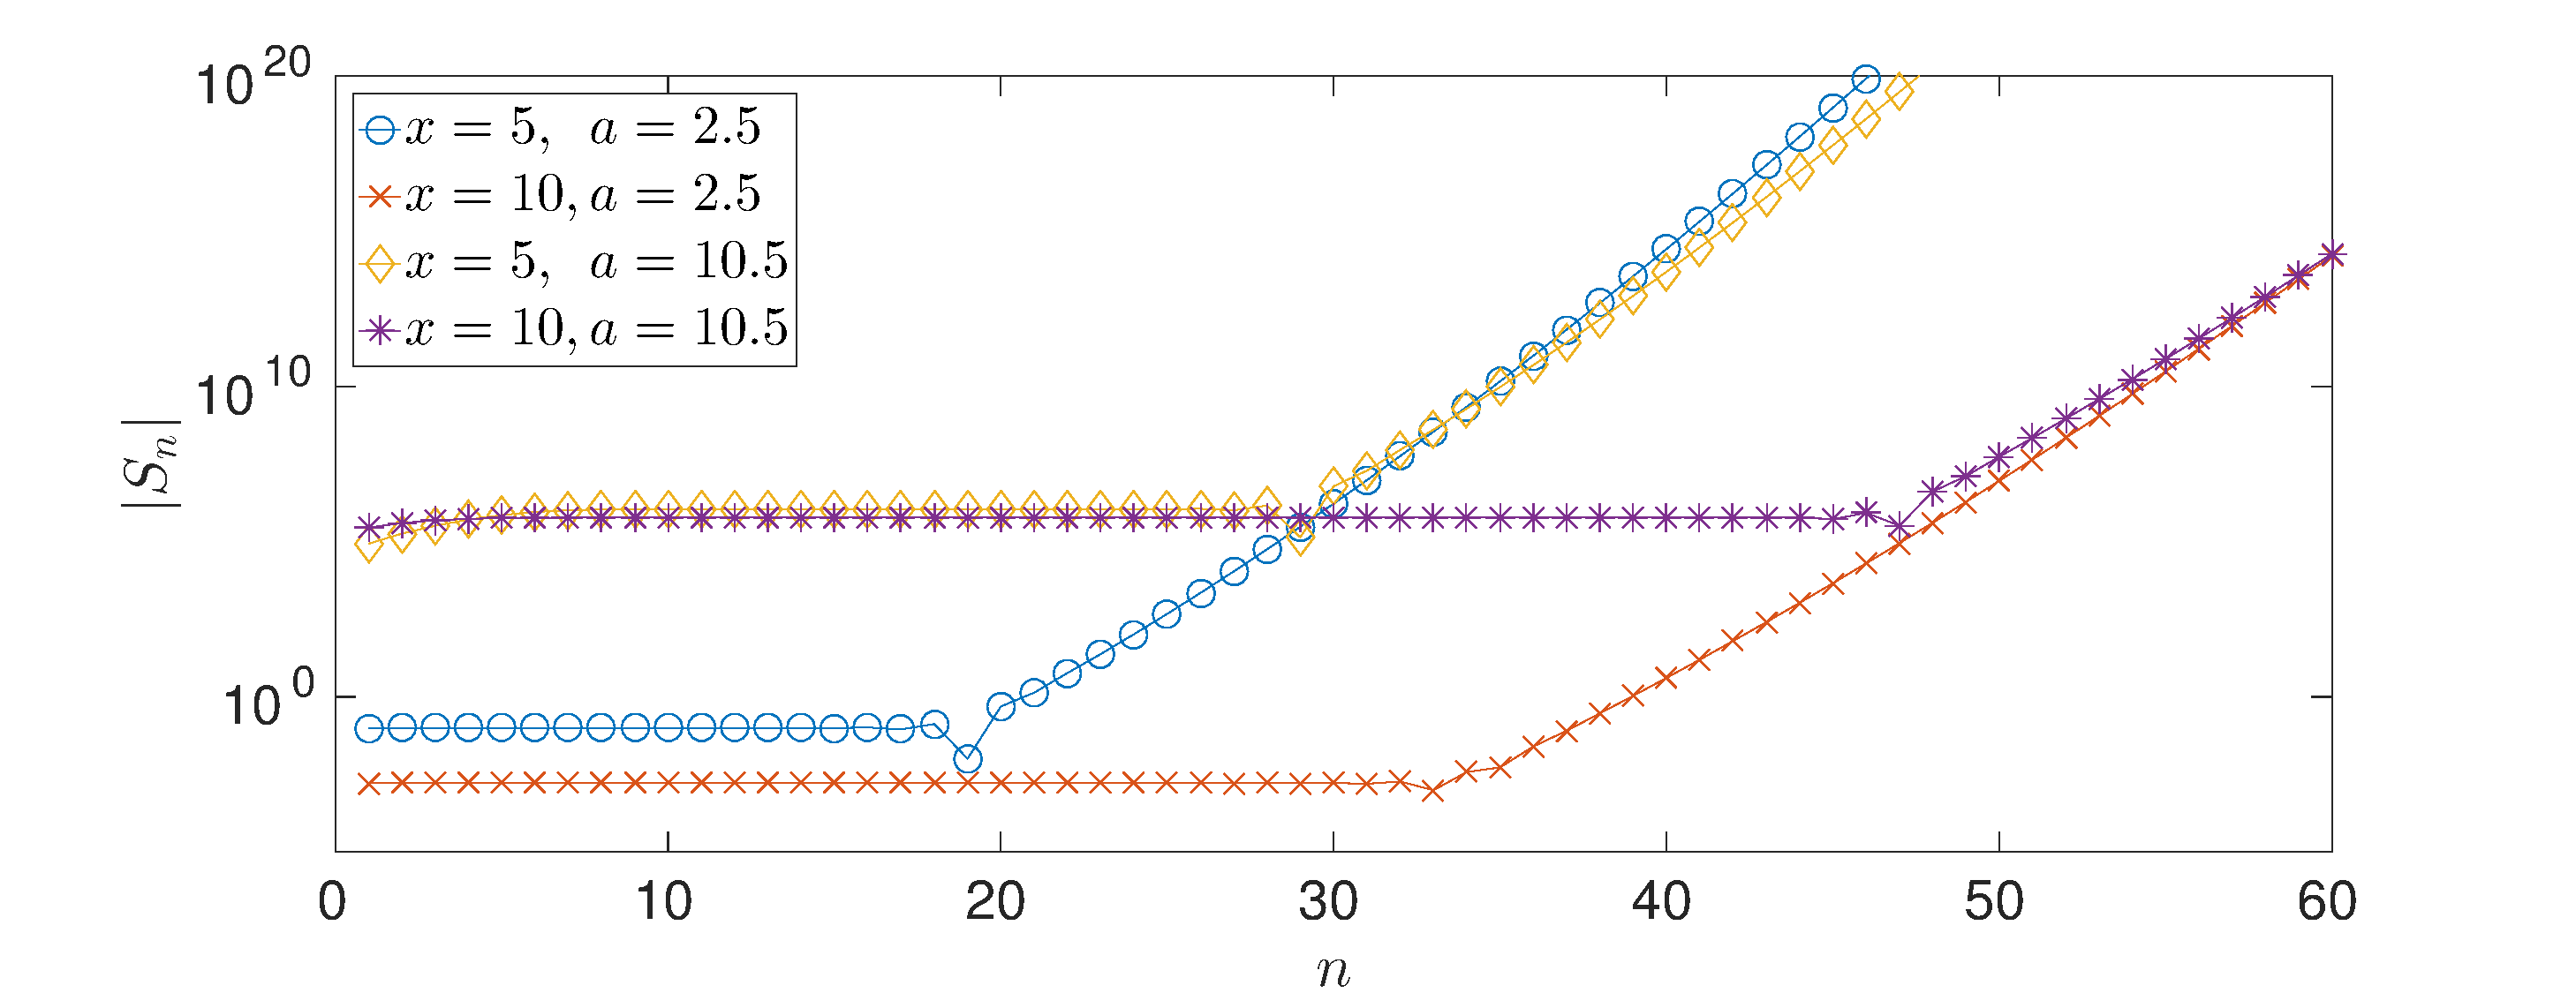
\includegraphics[width=1\textwidth]{Sn_a.pdf}
}
\caption{Logarithmic plot of $|S_n(x, a-1)|$ as a function of $n$
  for some different $x$ and $a$}.
\label{fig:Sn_a}
\end{figure}



\end{document}





%% På svenska ska citattecknet vara samma i både början och slut.
%% Använd två apostrofer (två enkelfjongar): ''.


%% Inkludera PDF-dokument
\includepdf[pages={1-}]{filnamn.pdf} %Filnamnet får INTE innehålla 'mellanslag'!

%% Figurer inkluderade som pdf-filer
\begin{figure}\centering
\centerline{ %centrerar även större bilder
\includegraphics[width=1\textwidth]{filnamn.pdf}
}
\caption{}
\label{fig:}
\end{figure}

%% Figurer inkluderade med xfigs "Combined PDF/LaTeX"
\begin{figure}\centering
\resizebox{.8\textwidth}{!}{\input{filnamn.pdf_t}}
\caption{}
\label{fig:}
\end{figure}

%% Figurer roterade 90 grader
\begin{sidewaysfigure}\centering
\centerline{ %centrerar även större bilder
\includegraphics[width=1\textwidth]{filnamn.pdf}
}
\caption{}
\label{fig:}
\end{sidewaysfigure}


%%Om man vill lägga till något i TOC
\stepcounter{section} %Till exempel en 'section'
\addcontentsline{toc}{section}{\Alph{section}\hspace{8 pt}Labblogg} 

